\chapter{The BEAVRS Benchmark}
\label{chap:beavrs}

The results presented in this thesis are based on models formed from the BEAVRS benchmark~\cite{horelik2013beavrs}. This chapter introduces the BEAVRS benchmark in Section~\ref{sec:beavrs-intro}, including a description of alteration made to the benchmark. Section~\ref{sec:beavrs-xs-gen} describes how cross-sections are generated for the benchmark. Finally, Section~\ref{sec:beavrs-models} details the particular models formed from cutouts of the BEAVRS model.

%%%%%%%%%%%%%%%%%%%%%%%%%%%%%%%%%%%%%%%%%%%%%%%%%%%%%%%%%%%%%%%%%%%%%%%%%%%%%%%%
\section{Introduction to the BEAVRS Benchmark}
\label{sec:beavrs-intro}

The BEAVRS benchmark~\cite{horelik2013beavrs} was released in 2013, representing a Westinghouse 4-loop nuclear power reactor. This reactor is representative of common \ac{PWR} designs in the United States. The benchmark contains core loadings and detector measurements for the first two cycles of operation, but this thesis concentrates on \ac{HZP} simulations at the beginning of the first cycle in an all rods out configuration.

The reactor contains 193 fuel assemblies. Each assembly contains a $17 \times 17$ lattice of fuel rods, guide tubes, and instrument tubes. The pin-pitch is 1.26 cm inside each assembly. All fuel rods within the same assembly contain uranium of the same enrichment. In the first cycle, three uranium enrichments are used: 1.6\%, 2.4\%, and 3.1\%. Wet annular burnable absorbers are present throughout the core to flatten the power distribution. The active fuel height is 365.76 cm. A radial description of the core is shown in Figure~\ref{fig:beavrs-assembly-enrichment}.

\begin{figure}[h!]
	\centering
	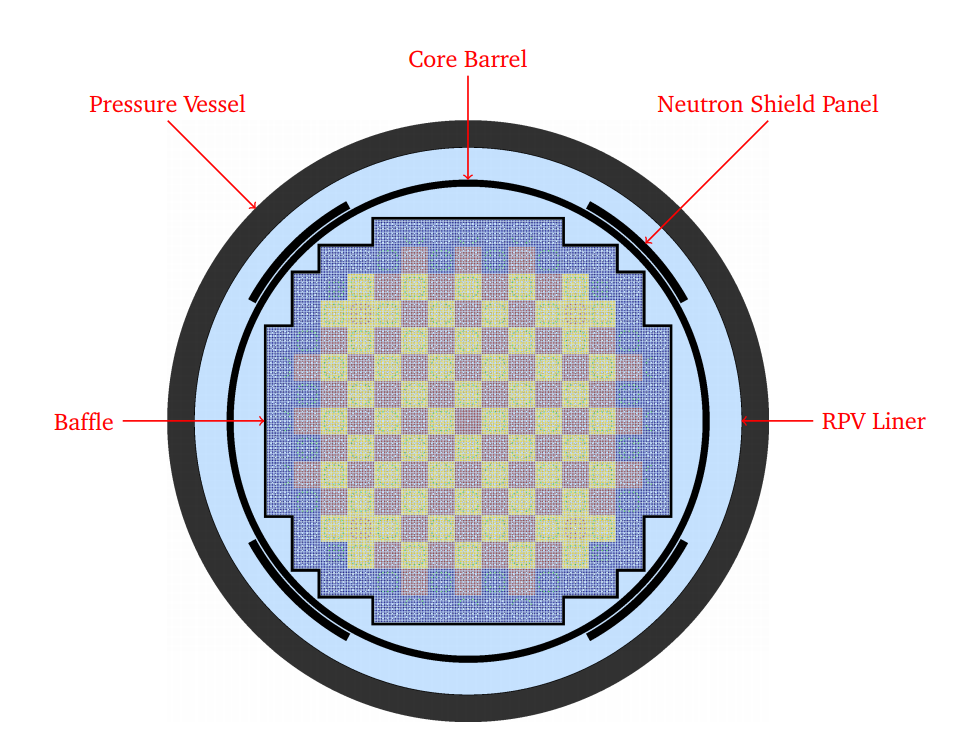
\includegraphics[width=\linewidth]{figures/beavrs-visual/beavrs-assembly-enrichment.png}
	\caption{A radial illustration of the BEAVRS benchmark with fuel pins colored by enrichment.}
	\label{fig:beavrs-assembly-enrichment}
\end{figure} 

One of the goals of this thesis is to simulate the BEAVRS benchmark using the explicit detail provided in the BEAVRS specification. However, in order to conduct uniform axial mesh refinement studies, the axial heights of material regions are altered such that each material discontinuity occurs at an even number of cm. The top and bottom grid spacers in the BEAVRS benchmark were defined to be 3.36 cm with intermediate grid spacers 5.72 cm. These lengths were altered to 2.0 cm and 6.0 cm, respectively. The starting height of the grid spacers were rounded to the nearest even integer. All other $z$-heights in the geometry were similarly rounded to the nearest even integer. The altering of axial heights allows regions to be formed which all have the same axial height, which simplifies axial uniform mesh refinement sensitivity studies. The altered axial heights are depicted in Figure~\ref{fig:fuel-rod-spec}. While these alterations do change the benchmark slightly, and therefore also change the computed solutions, these solutions are still very close to those of the true BEAVRS benchmark.

\begin{figure}[htbp]
	\centering
	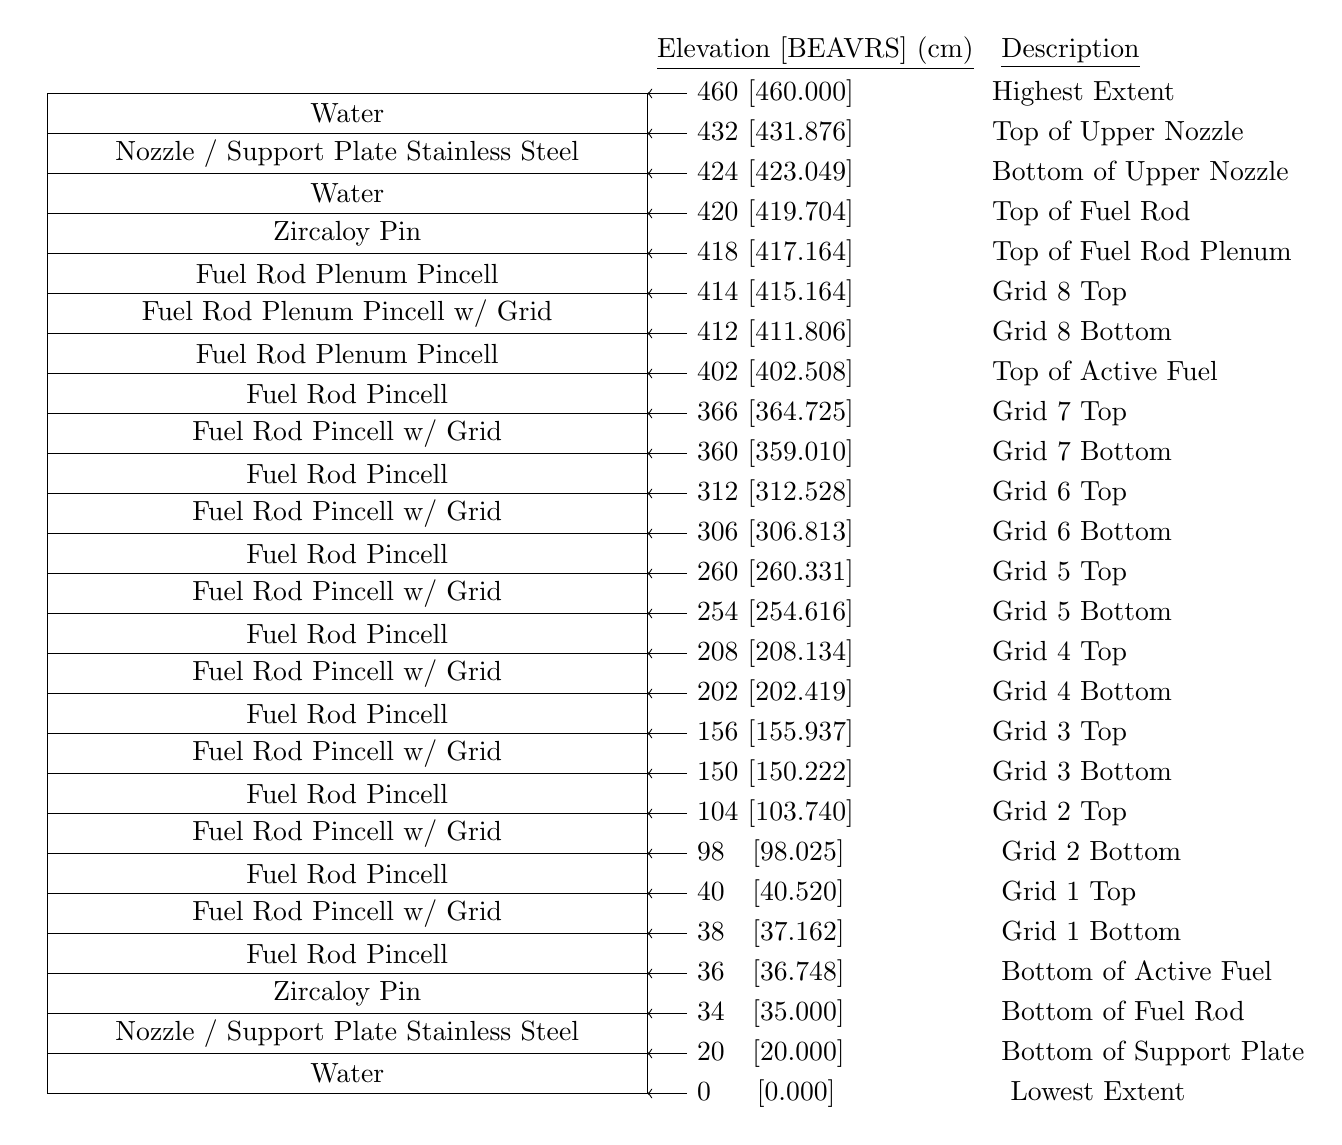
\begin{tikzpicture}[scale=1,x=1in,y=1in]
	\node[inner sep=0pt,
	text width=3 in,
	minimum size=0.2 in,
	draw=black,
	align=center,
	shift={(0,0.0)}] (n0) {Water};
	\draw[->] (1.7,-0.1) node[right,anchor=west] {0~~~~ [0.000] ~~~~~~~~~~~~~~~~~ Lowest Extent} -- (1.5,-0.1);
	\node[anchor=east] (s0) at (n0.west) {};
	\node[inner sep=0pt,
	text width=3 in,
	minimum size=0.2 in,
	draw=black,
	align=center,
	shift={(0,0.2)}] (n1) {Nozzle / Support Plate Stainless Steel};
	\draw[->] (1.7,0.1) node[right,anchor=west] {20~~ [20.000] ~~~~~~~~~~~~~~~ Bottom of Support Plate} -- (1.5,0.1);
	\node[inner sep=0pt,
	text width=3 in,
	minimum size=0.2 in,
	draw=black,
	align=center,
	shift={(0,0.4)}] (n2) {Zircaloy Pin};
	\draw[->] (1.7,0.3) node[right,anchor=west] {34~~ [35.000] ~~~~~~~~~~~~~~~ Bottom of Fuel Rod} -- (1.5,0.3);
	\node[inner sep=0pt,
	text width=3 in,
	minimum size=0.2 in,
	draw=black,
	align=center,
	shift={(0,0.6)}] (n3) {Fuel Rod Pincell};
	\draw[->] (1.7,0.5) node[right,anchor=west] {36~~ [36.748] ~~~~~~~~~~~~~~~ Bottom of Active Fuel} -- (1.5,0.5);
	\node[inner sep=0pt,
	text width=3 in,
	minimum size=0.2 in,
	draw=black,
	align=center,
	shift={(0,0.8)}] (n4) {Fuel Rod Pincell w/ Grid};
	\draw[->] (1.7,0.7) node[right,anchor=west] {38~~ [37.162] ~~~~~~~~~~~~~~~ Grid 1 Bottom} -- (1.5,0.7);
	\node[inner sep=0pt,
	text width=3 in,
	minimum size=0.2 in,
	draw=black,
	align=center,
	shift={(0,1.0)}] (n5) {Fuel Rod Pincell};
	\draw[->] (1.7,0.9) node[right,anchor=west] {40~~ [40.520] ~~~~~~~~~~~~~~~ Grid 1 Top} -- (1.5,0.9);
	\node[inner sep=0pt,
	text width=3 in,
	minimum size=0.2 in,
	draw=black,
	align=center,
	shift={(0,1.2)}] (n6) {Fuel Rod Pincell w/ Grid};
	\draw[->] (1.7,1.1) node[right,anchor=west] {98~~ [98.025] ~~~~~~~~~~~~~~~ Grid 2 Bottom} -- (1.5,1.1);
	\node[inner sep=0pt,
	text width=3 in,
	minimum size=0.2 in,
	draw=black,
	align=center,
	shift={(0,1.4)}] (n7) {Fuel Rod Pincell};
	\draw[->] (1.7,1.3) node[right,anchor=west] {104 [103.740] ~~~~~~~~~~~~~ Grid 2 Top} -- (1.5,1.3);
	\node[inner sep=0pt,
	text width=3 in,
	minimum size=0.2 in,
	draw=black,
	align=center,
	shift={(0,1.6)}] (n8) {Fuel Rod Pincell w/ Grid};
	\draw[->] (1.7,1.5) node[right,anchor=west] {150 [150.222] ~~~~~~~~~~~~~ Grid 3 Bottom} -- (1.5,1.5);
	\node[inner sep=0pt,
	text width=3 in,
	minimum size=0.2 in,
	draw=black,
	align=center,
	shift={(0,1.8)}] (n9) {Fuel Rod Pincell};
	\draw[->] (1.7,1.7) node[right,anchor=west] {156 [155.937] ~~~~~~~~~~~~~ Grid 3 Top} -- (1.5,1.7);
	\node[inner sep=0pt,
	text width=3 in,
	minimum size=0.2 in,
	draw=black,
	align=center,
	shift={(0,2.0)}] (n10) {Fuel Rod Pincell w/ Grid};
	\draw[->] (1.7,1.9) node[right,anchor=west] {202 [202.419] ~~~~~~~~~~~~~ Grid 4 Bottom} -- (1.5,1.9);
	\node[inner sep=0pt,
	text width=3 in,
	minimum size=0.2 in,
	draw=black,
	align=center,
	shift={(0,2.2)}] (n11) {Fuel Rod Pincell};
	\draw[->] (1.7,2.1) node[right,anchor=west] {208 [208.134] ~~~~~~~~~~~~~ Grid 4 Top} -- (1.5,2.1);
	\node[inner sep=0pt,
	text width=3 in,
	minimum size=0.2 in,
	draw=black,
	align=center,
	shift={(0,2.4)}] (n12) {Fuel Rod Pincell w/ Grid};
	\draw[->] (1.7,2.3) node[right,anchor=west] {254 [254.616] ~~~~~~~~~~~~~ Grid 5 Bottom} -- (1.5,2.3);
	\node[inner sep=0pt,
	text width=3 in,
	minimum size=0.2 in,
	draw=black,
	align=center,
	shift={(0,2.6)}] (n13) {Fuel Rod Pincell};
	\draw[->] (1.7,2.5) node[right,anchor=west] {260 [260.331] ~~~~~~~~~~~~~ Grid 5 Top} -- (1.5,2.5);
	\node[inner sep=0pt,
	text width=3 in,
	minimum size=0.2 in,
	draw=black,
	align=center,
	shift={(0,2.8)}] (n14) {Fuel Rod Pincell w/ Grid};
	\draw[->] (1.7,2.7) node[right,anchor=west] {306 [306.813] ~~~~~~~~~~~~~ Grid 6 Bottom} -- (1.5,2.7);
	\node[inner sep=0pt,
	text width=3 in,
	minimum size=0.2 in,
	draw=black,
	align=center,
	shift={(0,3.0)}] (n15) {Fuel Rod Pincell};
	\draw[->] (1.7,2.9) node[right,anchor=west] {312 [312.528] ~~~~~~~~~~~~~ Grid 6 Top} -- (1.5,2.9);
	\node[inner sep=0pt,
	text width=3 in,
	minimum size=0.2 in,
	draw=black,
	align=center,
	shift={(0,3.2)}] (n16) {Fuel Rod Pincell w/ Grid};
	\draw[->] (1.7,3.1) node[right,anchor=west] {360 [359.010] ~~~~~~~~~~~~~ Grid 7 Bottom} -- (1.5,3.1);
	\node[inner sep=0pt,
	text width=3 in,
	minimum size=0.2 in,
	draw=black,
	align=center,
	shift={(0,3.4)}] (n17) {Fuel Rod Pincell};
	\draw[->] (1.7,3.3) node[right,anchor=west] {366 [364.725] ~~~~~~~~~~~~~ Grid 7 Top} -- (1.5,3.3);
	\node[inner sep=0pt,
	text width=3 in,
	minimum size=0.2 in,
	draw=black,
	align=center,
	shift={(0,3.6)}] (n18) {Fuel Rod Plenum Pincell};
	\draw[->] (1.7,3.5) node[right,anchor=west] {402 [402.508] ~~~~~~~~~~~~~ Top of Active Fuel} -- (1.5,3.5);
	\node[inner sep=0pt,
	text width=3 in,
	minimum size=0.2 in,
	draw=black,
	align=center,
	shift={(0,3.8)}] (n19) {Fuel Rod Plenum Pincell w/ Grid};
	\draw[->] (1.7,3.7) node[right,anchor=west] {412 [411.806] ~~~~~~~~~~~~~ Grid 8 Bottom} -- (1.5,3.7);
	\node[inner sep=0pt,
	text width=3 in,
	minimum size=0.2 in,
	draw=black,
	align=center,
	shift={(0,4.0)}] (n20) {Fuel Rod Plenum Pincell};
	\draw[->] (1.7,3.9) node[right,anchor=west] {414 [415.164] ~~~~~~~~~~~~~ Grid 8 Top} -- (1.5,3.9);
	\node[inner sep=0pt,
	text width=3 in,
	minimum size=0.2 in,
	draw=black,
	align=center,
	shift={(0,4.2)}] (n21) {Zircaloy Pin};
	\draw[->] (1.7,4.1) node[right,anchor=west] {418 [417.164] ~~~~~~~~~~~~~ Top of Fuel Rod Plenum} -- (1.5,4.1);
	\node[inner sep=0pt,
	text width=3 in,
	minimum size=0.2 in,
	draw=black,
	align=center,
	shift={(0,4.4)}] (n22) {Water};
	\draw[->] (1.7,4.3) node[right,anchor=west] {420 [419.704] ~~~~~~~~~~~~~ Top of Fuel Rod} -- (1.5,4.3);
	\node[inner sep=0pt,
	text width=3 in,
	minimum size=0.2 in,
	draw=black,
	align=center,
	shift={(0,4.6)}] (n23) {Nozzle / Support Plate Stainless Steel};
	\draw[->] (1.7,4.5) node[right,anchor=west] {424 [423.049] ~~~~~~~~~~~~~ Bottom of Upper Nozzle} -- (1.5,4.5);
	\node[inner sep=0pt,
	text width=3 in,
	minimum size=0.2 in,
	draw=black,
	align=center,
	shift={(0,4.8)}] (n24) {Water};
	\draw[->] (1.7,4.7) node[right,anchor=west] {432 [431.876] ~~~~~~~~~~~~~ Top of Upper Nozzle} -- (1.5,4.7);
	\draw[->] (1.7,4.9) node[right,anchor=west] {460 [460.000] ~~~~~~~~~~~~~ Highest Extent} -- (1.5,4.9);
	\draw (1.5,5.1) node[right,anchor=west] {\underline{Elevation [BEAVRS] (cm)} ~ \underline{Description}};
	
	\end{tikzpicture}
	
	
	\caption[Fuel rod pincell axial specification]{Fuel rod pincell axial specification.\label{fig:fuel-rod-spec}}
\end{figure}


Although the BEAVRS model is defined inside a cylindrical geometry, a rectangular bounding geometry is often used in \ac{MOC} methods for cyclic tracking. Therefore, the BEAVRS model is modeled with a rectangular prism bounding the geometry. In the radial plane, the bounding dimensions are square with sides equal to 17 assembly widths. Since the BEAVRS model has a maximum of 15 assemblies along each $x$ and $y$ direction, this allows at least one assembly of radial reflector to be modeled outside the core. In addition, the corners have very deep water reflectors. In the axial direction, the BEAVRS benchmark is modeled over a height of 400 cm, from 20 cm to 420 cm in the model specification, allowing approximately 20 cm of axial reflector in each direction. Vacuum boundaries are assumed on all surfaces. 


%%%%%%%%%%%%%%%%%%%%%%%%%%%%%%%%%%%%%%%%%%%%%%%%%%%%%%%%%%%%%%%%%%%%%%%%%%%%%%%%
\section{Cross-Section Generation}
\label{sec:beavrs-xs-gen}

In this thesis, the same 70 group cross-section library is used for all results involving the BEAVRS benchmark or cutouts of the BEAVRS benchmark, except for rod insertion studies in which a separate 70 group cross-section library was formed in order to have accurate control rod material cross-sections. All cross-section libraries and group structures use the CASMO-4 energy group boundaries~\cite{edenius1995casmo}, as given in Appendix~\ref{app:energy-groups}. In this section, the process used to form cross-sections is thoroughly discussed.

Using direct Monte Carlo simulation of the BEAVRS benchmark with the OpenMC code, reaction rate tallies are generated for each unique material. These allow for the computation of multi-group cross-sections with the methodology discussed in Chapter~\ref{chap:mgxs} using the \texttt{mgxs} package implemented by Boyd~\cite{boyd2017thesis}. The Monte Carlo simulation used the JEFF-3.2 cross-section data at a temperature of 566.483K. 400 batches (300 inactive, 100 active) were simulated with $2 \times 10^8$ particles per batch to tally the 70 group cross-section library. The flux-limited transport correction described in Section~\ref{sec:transport-correction} is applied to the cross-sections using anisotropic scattering rate tallies. Note that using these tallies to form the transport correction introduces approximation since the true tallies should involve angular fluxes rather than scalar fluxes. Since the anisotropic scattering rate tallies could vary significantly between core and reflector regions, the water is split into two materials for which cross-sections are independently formed: core water and outer reflector water. In addition, a third water material is also formed near the support plate / nozzle as the isotopic composition differs due to boron concentration. Instrument tubes are also scattered through the core, causing the problem to not be quadrant symmetric. A plot of the BEAVRS benchmark colored by unique material region is shown in Figure~\ref{fig:beavrs-materials-radial}. In addition, an axial plot of the materials is shown in Figure~\ref{fig:beavrs-materials-axial}. Similarly the radial and axial material plots of a 1.6\% enriched fuel assembly are shown in Figure~\ref{fig:beavrs-single-assembly-materials-radial} and Figure~\ref{fig:beavrs-single-assembly-materials-axial}, respectively.


\begin{figure}[h!]
	\centering
	\includegraphics[width=\linewidth]{figures/beavrs-visual/materials-beavrs-radial.jpg}
	\caption{A radial view of the BEAVRS benchmark with regions colored by material.}
	\label{fig:beavrs-materials-radial}
\end{figure} 

\begin{figure}[h!]
	\centering
	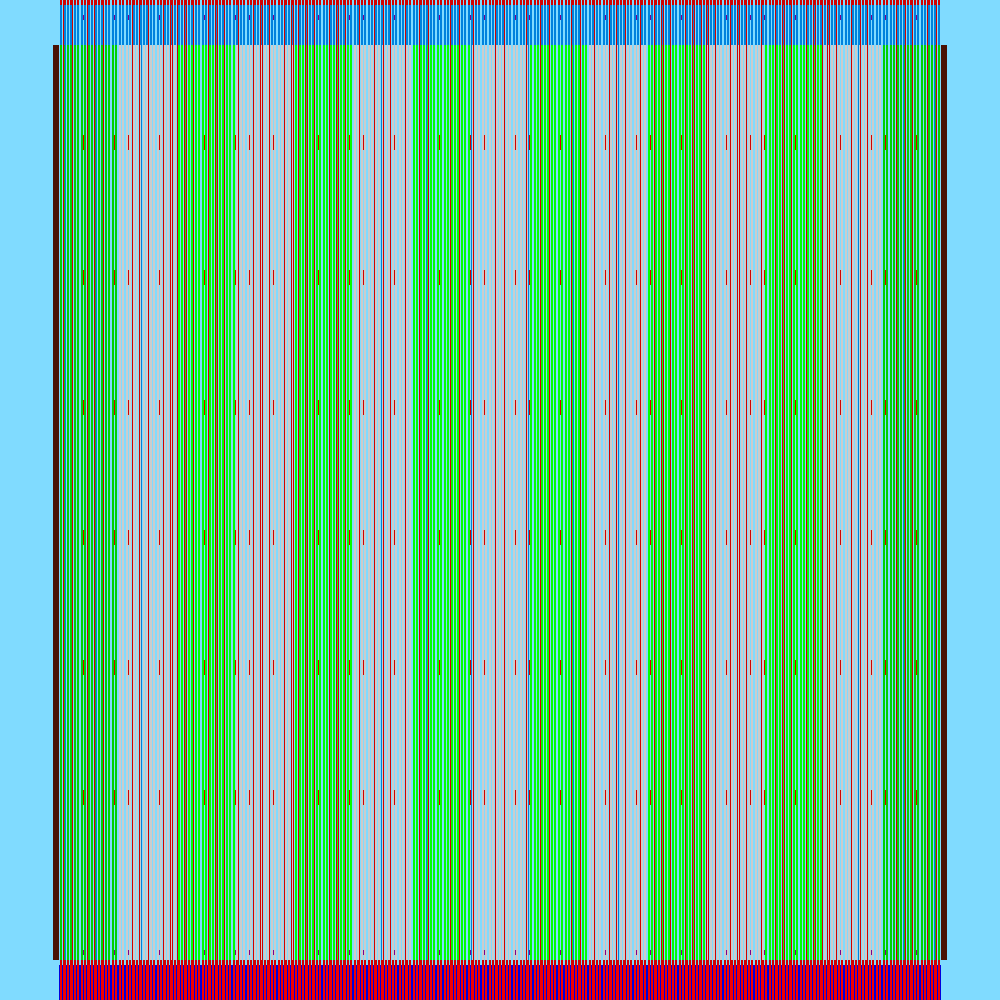
\includegraphics[width=\linewidth]{figures/beavrs-visual/materials-beavrs-axial.jpg}
	\caption{An axial view of the BEAVRS benchmark with regions colored by material.}
	\label{fig:beavrs-materials-axial}
\end{figure} 

\begin{figure}[h!]
	\centering
	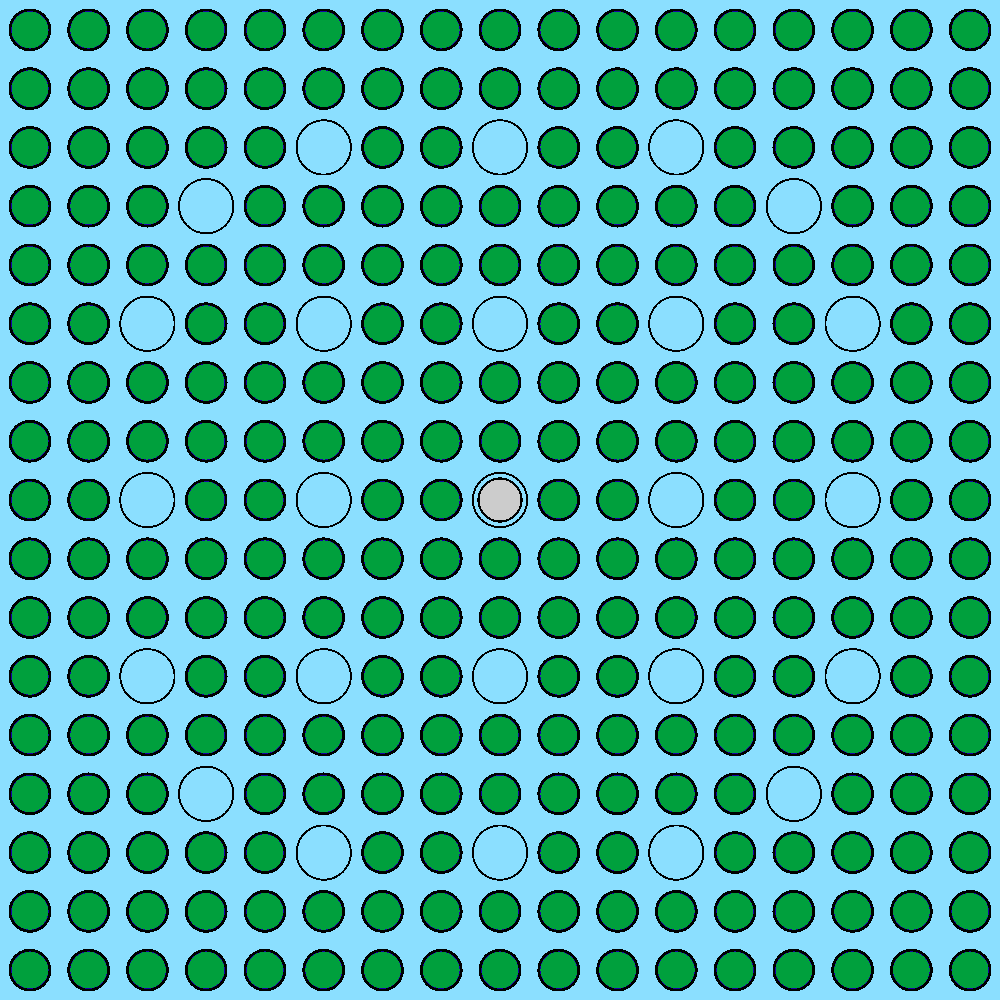
\includegraphics[width=0.65\linewidth]{figures/beavrs-visual/materials-single-assembly-radial.png}
	\caption{A radial view of the 1.6\% enriched fuel assembly in the BEAVRS benchmark with regions colored by material.}
	\label{fig:beavrs-single-assembly-materials-radial}
\end{figure} 

\begin{figure}[h!]
	\centering
	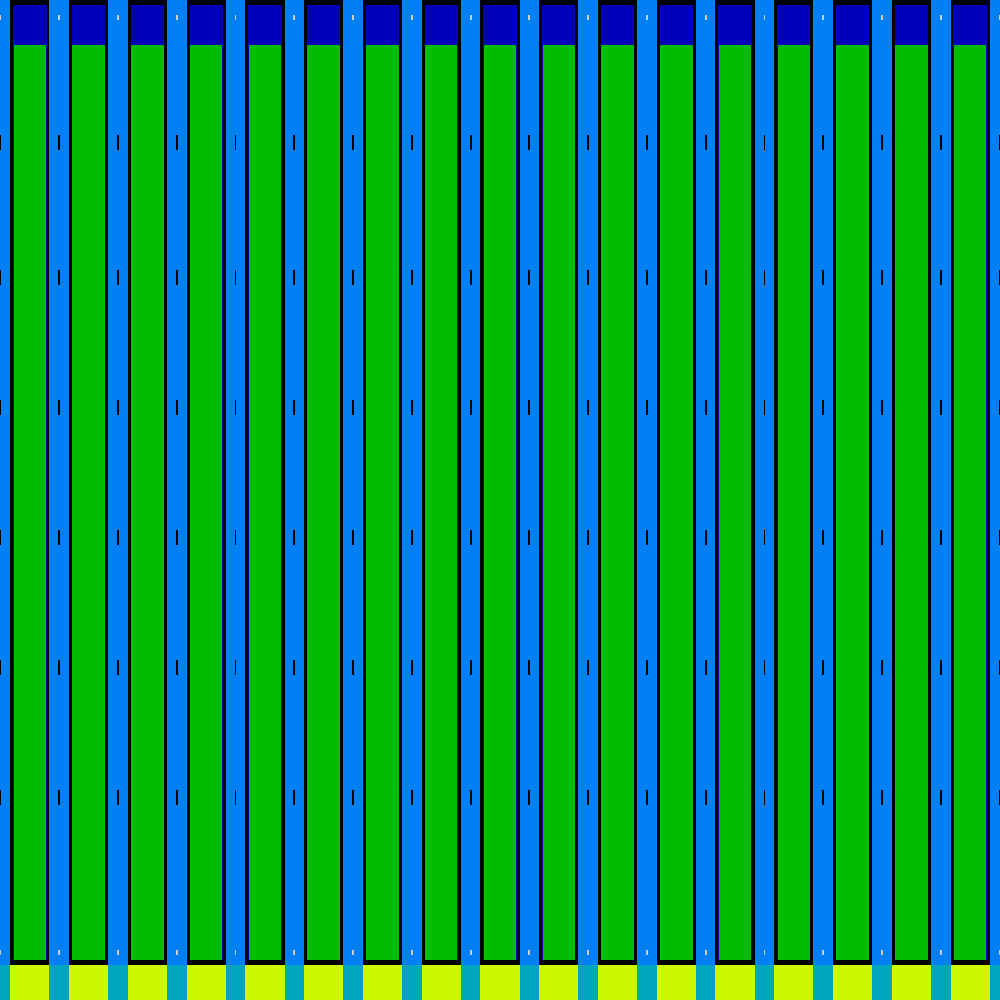
\includegraphics[width=0.65\linewidth]{figures/beavrs-visual/materials-single-assembly-axial.png}
	\caption{An axial view of 1.6\% enriched fuel assembly in the BEAVRS benchmark with regions colored by material.}
	\label{fig:beavrs-single-assembly-materials-axial}
\end{figure} 



\clearpage

The computed cross-sections were compared with CASMO-4 cross-sections and significant differences were found in the transport cross-section for water. In preliminary tests, the CASMO-4 multi-group cross-sections for core water were also able to much more accurately simulate the radial fission distribution. Therefore, instead of solely using the OpenMC \texttt{mgxs} cross-sections for core water which had an inaccurate transport correction, or solely using CASMO-4 cross-sections which are generated for more general problems, a new cross-section set was formed specifically for core water. Since CASMO-4 is a lattice physics code, it is designed to have accurate estimates of core water cross-sections. Therefore, the transport correction from CASMO-4 is used to modify the cross-sections formed by the OpenMC \texttt{mgxs} package. Specifically, the transport cross-section $\Sigma_{tr}^g$ for group $g$ is formed by computing
\begin{equation}
\Sigma_{tr}^g = \Sigma_{a}^g + \eta \left( \Sigma_{t}^g - \Sigma_{a}^g \right)
\end{equation}
where $\Sigma_{a}^g$ and $\Sigma_{t}^g$ are the associated absorption and total cross-sections formed by \texttt{mgxs}, respectively. The factor $\eta$ is computed by
\begin{equation}
\eta = \frac{\Sigma_{tr}^{g, \textbf{CASMO}} - \Sigma_{a}^{g, \textbf{CASMO}}}{\Sigma_{t}^{g, \textbf{CASMO}} - \Sigma_{a}^{g, \textbf{CASMO}}}
\label{eq:eta}
\end{equation}
where the \textbf{CASMO} superscript denotes CASMO-4 cross-sections. It is important to note that this is only done for core water. All other materials use the cross-sections formed directly from the \texttt{mgxs} package in OpenMC. A comparison of $\eta$ computed by OpenMC and by CASMO-4 for water is shown in Figure~\ref{fig:eta}.

\begin{figure}[h!]
	\centering
	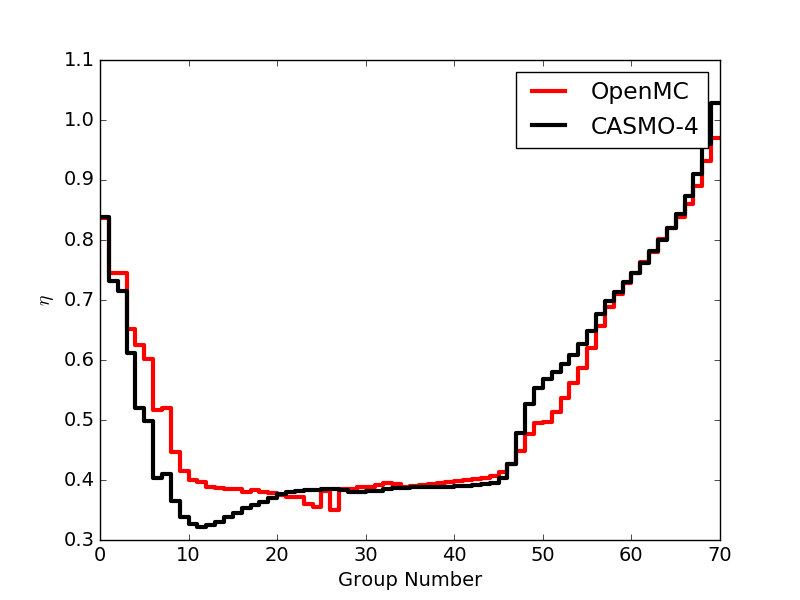
\includegraphics[width=0.7\linewidth]{figures/beavrs-visual/eta.png}
	\caption{A comparison of the $\eta$ factor defined in Eq.~\ref{eq:eta} for cross-sections generated with OpenMC and the CASMO-4 cross-sections for water in 70 energy groups.}
	\label{fig:eta}
\end{figure} 

\newpage
%%%%%%%%%%%%%%%%%%%%%%%%%%%%%%%%%%%%%%%%%%%%%%%%%%%%%%%%%%%%%%%%%%%%%%%%%%%%%%%%
\section{Description of BEAVRS Models}
\label{sec:beavrs-models}

All models which are simulated in this thesis are derived from cutouts of the BEAVRS benchmark with 70 group cross-sections. In past presentations, the 3D \ac{MOC} solver implemented in this thesis has been verified on a variety of simpler, conventional reactor physics models~\cite{physor2016shaner, physor2016otf}. The BEAVRS benchmark represents a far more computationally demanding challenge, especially with a 70 group cross-section library. Cutouts are formed in order to evaluate smaller problems which are representative of computational performance or physical behavior of the large full core problem.

\subsection{Full Core 3D Model}
\label{sec:beavrs-3D}

The first model is the full core 3D BEAVRS model, incorporating all the details discussed in previous sections. The simulation of this model directly corresponds with the OpenMC simulations from which the cross-sections are derived. The objective of this thesis is to accurately simulate this model. However, due to the large computational cost of simulating this model, only a minimal number of tests can be conducted. Therefore, more computationally feasible, smaller cutouts are formed in order to test computational and physical behavior before running the 3D full core case.


\subsection{Full Core 2D Model}
\label{sec:beavrs-2D}

A 2D extruded cutout of the reactor is formed in order to determine the physical behavior of the BEAVRS model in the radial direction. This cutout is taken from a 10 cm axial interval over which there are no grid spacers. Reflective boundary conditions are placed on the top and bottom of the problem. While this model lacks any axial variation, it still contains all radial detail except grid spacers. Due to the lack of axial detail, 2D \ac{MOC} and 3D \ac{MOC} simulations with sufficient parameter refinement should produce equivalent solutions. Only this model and the full core 3D model contain the full radial water reflector. Therefore, this model is very useful in determining the effect of large radial water reflectors. 

\subsection{Single Assembly Model}
\label{sec:beavrs-single-assembly}

A single assembly model is formed which represents the full axial detail of a single 1.6\% enriched fuel assembly. While this model lacks radial water reflectors, it contains the full axial detail of the full core problem, including grid spacers. Outside the core, full geometrical detail is also captured including support plate / nozzles and, most notably, water reflectors of approximately 20 cm above and below the fuel. Reflective boundaries are placed on the $x$ and $y$ boundaries. Physically, this is equivalent to an infinite 2D lattice of 1.6\% enriched fuel assemblies. Vacuum boundaries remain on the top and bottom of this model. Since this problem is significantly less computationally expensive than the full core models (both 2D and 3D), it allows for rigorous parameter refinement and convergence studies.

\subsection{Single Assembly Model without Reflectors}
\label{sec:trunc-single-assembly}

In addition to the single assembly model, a single assembly model without reflectors is also formed which contains all the detail of the single assembly model, but without the axial water reflectors. Specifically, 20 cm are removed from both the bottom and top of the model, resulting in a model that only covers the active fuel and is 360 cm tall. Axial boundaries still have vacuum boundary conditions. Comparison with the single assembly model described in Section~\ref{sec:beavrs-single-assembly} allows for the effect of axial water reflectors to be directly tested.

\subsection{SDSA Model}
\label{sec:sdsa}

The Single Domain Single Assembly (SDSA) model represents a 20 cm tall cutout within the single assembly model which contains no grid spacers. Reflective boundary conditions are imposed on all surfaces. Since this problem is far reduced in size, it allows for rigorous performance testing. In Chapter~\ref{chap:domain-decomposition}, spatial domain decomposition is introduced in which the geometry is split into equal sized domains in which each computational node is expected to handle one domain. When simulating the BEAVRS benchmark with domain decomposition, the expected domain size is the size of the SDSA model. Therefore, this model allows for realistic on-node performance characterization of the BEAVRS benchmark without needing to run the large full core problem.

\subsection{Short Single Assembly Model}
\label{sec:short-single-assembly}

Similar to the SDSA model, the short single assembly model is created which allows for more feasible testing due to its far reduced size. This model is the same as the SDSA model except it is only 10 cm in axial height and contains 3.1\% enriched fuel. This enrichment is the highest enrichment found in the cycle 1 BEAVRS model. The greater fuel enrichment allows for slightly larger gradients with a flux peak in the moderator. The primary focus of this model is to test in-core radial mesh sensitivity.


\subsection{Rodded Single Assembly Model}
\label{sec:rodded-single-assembly}

The rodded single assembly model is the only model which uses a geometry not explicitly found in the full core 3D BEAVRS model. The model is constructed in the same way as the single assembly model described in Section~\ref{sec:beavrs-single-assembly}, but with 3.1\% enriched fuel and with all rods inserted, covering approximately half of the active fuel height. The axial zones of guide tubes containing the inserted control rods are shown in Figure~\ref{fig:control-rod-spec}.

\begin{figure}[htbp]
	\centering
	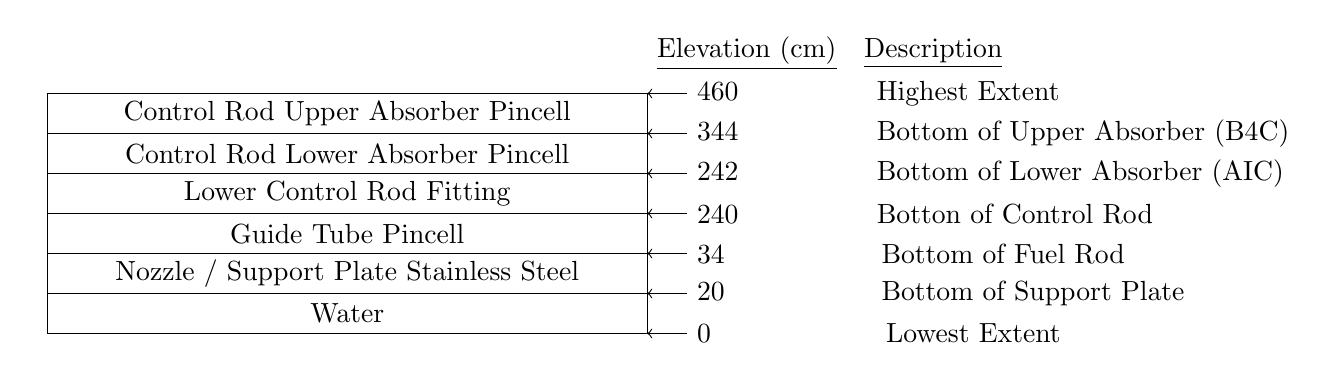
\begin{tikzpicture}[scale=1,x=1in,y=1in]
	\node[inner sep=0pt,
	text width=3 in,
	minimum size=0.2 in,
	draw=black,
	align=center,
	shift={(0,0.0)}] (n0) {Water};
	\draw[->] (1.7,-0.1) node[right,anchor=west] {0 ~~~~~~~~~~~~~~~~~ Lowest Extent} -- (1.5,-0.1);
	\node[anchor=east] (s0) at (n0.west) {};
	\node[inner sep=0pt,
	text width=3 in,
	minimum size=0.2 in,
	draw=black,
	align=center,
	shift={(0,0.2)}] (n1) {Nozzle / Support Plate Stainless Steel};
	\draw[->] (1.7,0.1) node[right,anchor=west] {20 ~~~~~~~~~~~~~~~ Bottom of Support Plate} -- (1.5,0.1);
	\node[inner sep=0pt,
	text width=3 in,
	minimum size=0.2 in,
	draw=black,
	align=center,
	shift={(0,0.4)}] (n2) {Guide Tube Pincell};
	\draw[->] (1.7,0.3) node[right,anchor=west] {34 ~~~~~~~~~~~~~~~ Bottom of Fuel Rod} -- (1.5,0.3);
	\node[inner sep=0pt,
	text width=3 in,
	minimum size=0.2 in,
	draw=black,
	align=center,
	shift={(0,0.6)}] (n3) {Lower Control Rod Fitting};
	\draw[->] (1.7,0.5) node[right,anchor=west] {240 ~~~~~~~~~~~~~ Botton of Control Rod} -- (1.5,0.5);
	
	\node[inner sep=0pt,
	text width=3 in,
	minimum size=0.2 in,
	draw=black,
	align=center,
	shift={(0,0.8)}] (n4) {Control Rod Lower Absorber Pincell};
	\draw[->] (1.7,0.7) node[right,anchor=west] {242 ~~~~~~~~~~~~~ Bottom of Lower Absorber (AIC)} -- (1.5,0.7);
	\node[inner sep=0pt,
	text width=3 in,
	minimum size=0.2 in,
	draw=black,
	align=center,
	shift={(0,1.0)}] (n5) {Control Rod Upper Absorber Pincell};
	\draw[->] (1.7,0.9) node[right,anchor=west] {344 ~~~~~~~~~~~~~ Bottom of Upper Absorber (B4C)} -- (1.5,0.9);
	
	\draw[->] (1.7,1.1) node[right,anchor=west] {460 ~~~~~~~~~~~~~ Highest Extent} -- (1.5,1.1);
	\draw (1.5,1.3) node[right,anchor=west] {\underline{Elevation (cm)} ~ \underline{Description}};
	
	\end{tikzpicture}
	
	
	\caption[Control Rod Insertion]{Control rod pincell axial specification for the single assembly control rod insertion model.\label{fig:control-rod-spec}}
\end{figure}


The large control rod insertion causes significant gradients within the axial scalar flux distribution, allowing for robust testing of 3D \ac{MOC} on problems with significant axial variation. As mentioned previously, this model uses a separate cross-section library. Instead of simulating the all rods out configuration, which lacks control rods within the core, the rodded single assembly model is explicitly simulated in OpenMC to form cross-section estimates. This allows reasonable estimates of control rod material cross-sections.

%\newpage
%\vfill
%\begin{highlightsbox}[frametitle=Highlights]
%	\begin{itemize}
%		\item The BEAVRS benchmark represents a traditional \ac{PWR} reactor encompassing all relevant radial and axial detail
%		\item The BEAVRS model is simulated within a radially square bounding box, leading to large corner reflector regions
%		\item A 70 group cross-section library is formed through direct simulation of the BEAVRS benchmark in Monte Carlo using the OpenMC \texttt{mgxs} package with a combination of CASMO-4 and in-scatter transport corrections
%		\item Cutouts of the BEAVRS model allow for physics and computational behavior to be tested with much lower computational cost
%		\item A rodded single assembly model is created to test the effect of large axial variation, for which a separate cross-section library is generated in order to accurately capture control rod properties
		
%	\end{itemize}
%\end{highlightsbox}
%\vfill

